\documentclass[a4paper, 12pt, twoside, openright]{article}

\usepackage[utf8]{inputenc}
\usepackage[T1]{polski}
\usepackage{helvet}
\usepackage{graphicx}
\usepackage{color}
\usepackage[top=1.3in,bottom=1.3in,right=1in,left=1in,headheight=95pt,headsep=-0.5cm]{geometry}


\begin{document}

% =====  STRONA TYTULOWA  ====

\thispagestyle{empty}
\vspace*{-0.6in}
%% ------------------------ NAGLOWEK STRONY =======================------

\includegraphics[height=37.5mm]{logo_agh}\\
\rule{30mm}{0pt}
{\large\textsf{Wydział Fizyki i Informatyki Stosowanej}}\\
\rule{\textwidth}{3pt}\\
\rule[2ex]
{\textwidth}{1pt}\\
\vspace{7ex}
\begin{center}
{\bf\LARGE\textsf{Praca inżynierska}}\\
\vspace{13ex}
% ======================= IMIE I NAZWISKO =======================----
{\bf\Large\textsf{Klaudia Fil}}\\
\vspace{3ex}
{\sf \small kierunek studiów:} {\bf\small\textsf{informatyka stosowana}}\\
\vspace{15ex}
%% ------------------------ TYTUL PRACY =======================-----------
{\bf\huge\textsf{Problem chińskiego listonosza\\ w sieci ulic w Krakowie}}\\
\vspace{14ex}
%% ------------------------ OPIEKUN PRACY =======================---------
{\sf \Large Opiekun:} {\bf\Large\textsf{dr hab. inż. Przemysław Gawroński}}\\
\vspace{22ex}
\textsf{\bf\large\textsf{Kraków, styczeń 2021}}
\end{center}


\newpage

%% =====  Oświadczenie =========
\begin{center}
	{\bf\large\textsf{Oświadczenie studenta}}
\end{center}


{\sf 
	Uprzedzony(-a) o odpowiedzialności karnej na podstawie art. 115 ust. 1 i 2 ustawy z dnia 4 lutego 1994 r. o prawie autorskim i prawach pokrewnych (t.j. Dz. U. z 2018 r. poz. 1191 z późn. zm.): „Kto przywłaszcza sobie autorstwo albo wprowadza w błąd co do autorstwa całości lub części cudzego utworu albo artystycznego wykonania, podlega grzywnie, karze  ograniczenia wolności albo pozbawienia wolności do lat 3. Tej samej karze podlega, kto rozpowszechnia bez podania nazwiska lub pseudonimu twórcy cudzy utwór w wersji oryginalnej albo w postaci opracowania, artystyczne wykonanie albo publicznie zniekształca taki utwór, artystyczne wykonanie, fonogram, wideogram lub nadanie.”, a także uprzedzony(-a) o odpowiedzialności dyscyplinarnej na podstawie art. 307 ust. 1 ustawy z dnia 20 lipca 2018 r. Prawo o szkolnictwie wyższym i nauce (Dz. U. z 2018 r. poz. 1668 z późn. zm.) „Student podlega odpowiedzialności dyscyplinarnej za naruszenie przepisów obowiązujących w uczelni oraz za czyn uchybiający godności studenta.”, oświadczam, że niniejszą pracę dyplomową wykonałem(-am) osobiście i samodzielnie i nie korzystałem(-am) ze źródeł innych niż wymienione w pracy

\bigskip

	Jednocześnie Uczelnia informuje, że zgodnie z art. 15a ww. ustawy o prawie autorskim i prawach pokrewnych Uczelni przysługuje pierwszeństwo w opublikowaniu pracy dyplomowej studenta. Jeżeli Uczelnia nie opublikowała pracy dyplomowej w terminie 6 miesięcy od dnia jej obrony, autor może ją opublikować, chyba że praca jest częścią utworu zbiorowego. Ponadto Uczelnia jako podmiot, o którym mowa w art. 7 ust. 1 pkt 1 ustawy z dnia 20 lipca 2018 r. — Prawo o szkolnictwie wyższym i nauce (Dz. U. z 2018 r. poz. 1668 z późn. zm.), może korzystać bez wynagrodzenia i bez konieczności uzyskania zgody autora z utworu stworzonego przez studenta w wyniku wykonywania obowiązków związanych z odbywaniem studiów, udostępniać utwór ministrowi właściwemu do spraw szkolnictwa wyższego i nauki oraz korzystać z utworów znajdujących się w prowadzonych przez niego bazach danych, w celu sprawdzania z wykorzystaniem systemu antyplagiatowego. Minister właściwy do spraw szkolnictwa wyższego i nauki może korzystać z prac dyplomowych znajdujących się w prowadzonych przez niego bazach danych w zakresie niezbędnym do zapewnienia prawidłowego utrzymania i rozwoju tych baz oraz współpracujących z nimi systemów informatycznych.}

\vspace{15ex}

\begin{center}
\begin{tabular}{lr}
~~~~~~~~~~~~~~~~~~~~~~~~~~~~~~~~~~~~~~~~~~~~~~~~~~~~~~~~~~~~~~~~~ &
................................................................. \\
~ & {\sf (czytelny podpis)} \\
\end{tabular}
\end{center}

%% =====  TYL STRONY TYTULOWEJ   ====


%% ============ OCENA OPIEKUNA =============
\newpage
\linespread{1.3}
\selectfont

\hspace*{\fill}\large{Ocena merytoryczna opiekuna}

\vspace{85mm}

%% ============ OCENA RECENZENTA =============
\newpage
\linespread{1.3}
\selectfont

\hspace*{\fill}\large{Ocena merytoryczna recenzenta}

\vspace{85mm}


%% ====== SPIS TRESCI ==========
\newpage
\tableofcontents


%=======================- 1 =======================
\newpage
\section{Wstęp}
\subsection{Wprowadzenie}
	\indent\par
	Szeroko pojęty problem związany z wyznaczaniem trasy (ang. General Routing Problem) zdefiniowano jako szukanie drogi o minimalnym koszcie, która dodatkowo musi spełniać uwzględnione w planowaniu wymagania\cite{varianntsCPP}.
	Skupiając się na praktycznym aspekcie GRP należy wziąć pod uwagę jeden z bardziej znanych przypadków rozważań - problem chińskiego listonosza (ang.Chinese Postman Problem)\cite{arcRoutingProblemsPart1}. 


	W życiu codziennym wiele zawodów związanych jest wyznaczaniem trasy na tle procesów logistycznych, wśród nich różnego rodzaju dostawca, kurier czy właśnie listonosz. Ich szlakiem docelowym jest droga zawierająca w sobie każdą ulicę danego obszaru przynajmniej raz. Optymalnym rozwiązaniem CPP byłoby uniknięcie ponownych przejść jedną ścieżką, jednak w sytuacjach rzeczywistych jest to często niemożliwe.

\subsection{Cel pracy}
	\indent\par
	Celem pracy dyplomowej jest zaimplementowanie dwóch algorytmów, rozwiązujących kwestię znajdowania pełnej ścieżki z cyklem zamkniętym na grafie spójnym, przy optymalizacji kosztów przemieszczania się, co sprowadza się do CPP. 
	Rozpatrzono w niej przypadki rzeczywiste, gdzie w powstałych z mapy Krakowa grafach mieszanych (ang. Mixed Graph) oraz nieskierowanych (ang. Undirected Graph), znajdowana jest najlepsza droga dla listonosza\cite{mixedGraph}.


	Jeden z algorytmów przedstawiony w pracy dedykowany jest MG. Swoje zastosowanie ma, kiedy przebieg trasy listonosza uwarunkowany jest czynnikami zewnętrznymi tj. drogami jedno- lub dwukierunkowymi. 
	W przypadku pieszego ruchu, w którym sposób przejścia jest  dowolny, problem dotyczy UG. Zaimplementowano dla niego drugi z schematów umożliwiający wyznaczenie najbardziej efektywnej trasy. Graf rzeczywisty tworzony jest z małych fragmentów miasta, dlatego założono, że poruszać się będzie na nim tylko jeden listonosz. 


	Dla sprawdzenia poprawności oraz wyznaczenia złożoności algorytmów wygenerowano losowe sieci, które umożliwiły szersze ich przetestowanie. 
	Kolejne etapy trasy naniesiono na graf, co pozwoliło na graficzne prześledzenie działania programów.


\subsection{Graf rzeczywisty}\label{grafRzecz}
	\indent\par
	Algorytmy docelowo szukają optymalnej trasy na planie miasta Kraków. Poprawne ich zastosowanie wymaga konwersji mapy na postać grafową. 
	
	\begin{figure}[htb]
			\centering
			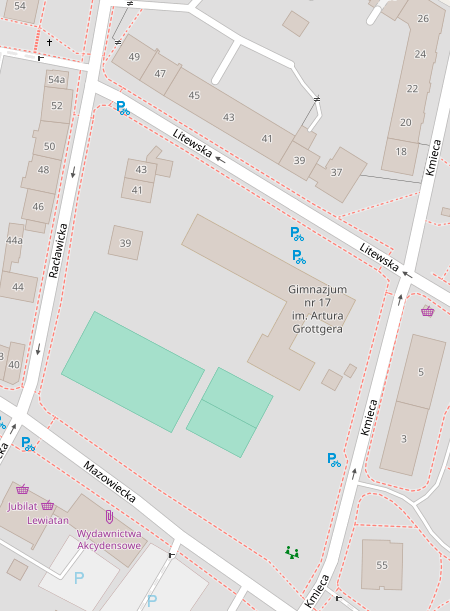
\includegraphics[width=0.5\textwidth]{OSM1}
			\caption[]{Fragment mapy Krakowa\footnotemark}
			\label{osm1}
	\end{figure}
	
	\footnotetext{Zrzut ekranu z strony https://www.openstreetmap.org/}

	Przetwarzając mapę z rysunku \ref{osm1}. formujemy graf, którego krawędzie odpowiadają ulicom, a wierzchołki reprezentują zarówno budynki, jak i istotne elementy dróg: skrzyżowania i strategiczne punkty trasy, które to potrzebne są do idealnego przeprowadzenia ulicy, czyli uwzględnienia zakrętów lub nieliniowych fragmentów drogi.

	\begin{figure}[htb]
		\centering
		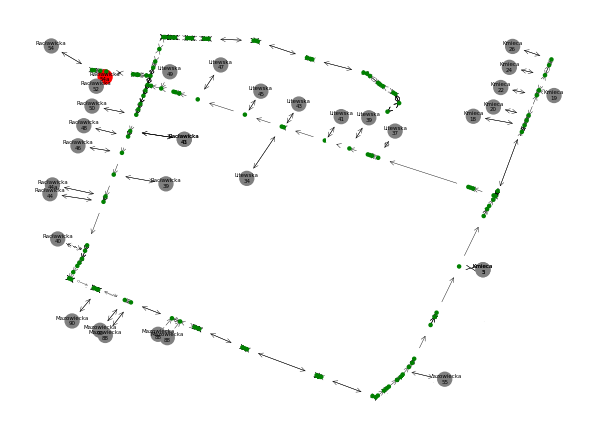
\includegraphics[width=0.9\textwidth]{OSM1graf}
		\caption[]{Graf rzeczywisty MG stworzony z mapy z rysunku \ref{osm1}.}
		\label{osm1G}
	\end{figure}
	
	Program odpowiedzialny za generowanie grafu, przy pobieraniu danych z bazy OpenStreetMap, filtruje odpowiednie informacje o obiektach i znajduje placówkę pocztową (o ile taka istnieje na danych fragmencie miasta) dzięki konkretnym tagom\cite{osmPropertis}. W przypadku wybrania fragmentu mapy, gdzie nie ma poczty, to miano nadawane jest losowo wybranej nieruchomości.
	
	Wierzchołki w grafie podpisano rzeczywistymi adresami oraz oznaczono różnymi kolorami, w celu zwiększenia czytelności. Placówkę pocztową przedstawiono na czerwono, zwykłe budynki mieszkalne na szaro. Natomiast wierzchołki będące fragmentami drogi pokolorowano na zielono oraz zmniejszono ich rozmiar względem pozostałych.
	
	Analizując kierunki dróg na rysunku \ref{osm1}. można zauważyć, że wpływają one na budowę grafu rzeczywistego z rysunku \ref{osm1G}., który w przypadku kiedy listonosz porusza się np. samochodem jest MG. Dla pieszej podróży  określono go jako UG.

\subsection{Problemu chińskiego listonosza}
	\indent\par
	....................
%	Problem chińskiego listonosza (CPP) jest jedynym z podstawowych zagadnień związanych z wyznaczaniem trasy. Swoją nazwę zawdzięcza chińskiemu matematykowi, który jako pierwszy go sformułował. Miał on dostarczyć wszystkie przesyłki nie nadkładając niepotrzebnie drogi i powrócić na pocztę. 
%	Patrząc przez pryzmat przypadku rzeczywistego (\ref{grafRzecz}) CPP sprowadza się do procesu wyboru najlepszej ścieżki w sieci dróg

\subsection{Ścieżka Eulera}
\indent\par
............
\cite{mixedNetworksCPP}
\cite{MatchingEulertourAsCPP}

\subsection{Sieci złożone}
\subsubsection{Sieć Barabási–Albert}
\indent\par
.................
\subsubsection{Sieć Watts–Strogatz}
\indent\par
....................

% ======================= 2 =======================
\newpage
\section{Narzędzia}
\subsection{Język Python}
\indent\par
..............



\subsection{Biblioteki}
\indent\par

\subsubsection{Networkx}
\indent\par
.............

\subsubsection{Matplotlib}
\indent\par
.............



\subsection{Narzędzia pomocnicze}
\indent\par
\subsubsection{OpenStreetMap}
\subsubsection{Github}
\indent\par
.............




%======================= 3 =======================
\newpage
\section{Algorytmy i implementacja}
\indent\par
........................




\subsection{Modyfikacja do grafu Eulera}
\indent\par
........................

\subsection{Implementacja grafu rzeczywistego}
\indent\par
........................

\subsection{Algorytm Fleury’ego}
\indent\par
........................


\subsection{Algorytm Hierholzera}
\indent\par
........................




% ======================= 4 =======================
\newpage
\section{Wyniki}
\par\indent
........................



% ======================= 5 =======================
\newpage
\section{Podsumowanie}
\indent\par
........................



% ======================= LITERARATURA =======================
\newpage
\begin{thebibliography}{99}
	
	% 1.1
	\bibitem{varianntsCPP}
		Gordenko M.K., Avdoshin S.M. \textit{The Variants of Chinese Postman Problems and Way of Solving through Transformation into Vehicle Routing Problems.} Trudy ISP RAN/Proc. ISP RAS, vol. 30, issue 3, s. 221-232, 2018
	
	\bibitem{arcRoutingProblemsPart1}
		H. A. Eiselt, M. Gendreau, G. Laporte, \textit{Arc Routing Problems, Part I: The Chinese Postman Problem}  Institute for Operations Research and the Management Sciences (INFORMS), 1995
	
	\bibitem{mixedGraph}Beck, M. Blado, D. Crawford, J. Jean-Louis, T. Young, M. \textit{On weak chromatic polynomials of mixed graphs}, Graphs and Combinatorics, 2013

	% 1.3	
	\bibitem{osmPropertis} https://wiki.openstreetmap.org/wiki/Category:Properties [dostęp: 20.12.2020]	

	% 1.5
	\bibitem{mixedNetworksCPP} W.L. Pearn, J.B. Chou. \textit{Improved solutions for the Chinese postman problem on mixed networks}. Computers\&Operations Research, s. 819–827, 1999
	
	\bibitem{MatchingEulertourAsCPP} J.Edmonds, E.L.Johnson.  \textit{Matching Euler tours and the Chinese postman problem}. Mathematical Programming, s. 88–124, 1973
	
	\bibitem{cormen}
		Thomas H. Cormen, Charles E. Leiserson, Ronald L. Rivest, Clifford Stein, \textit{Wprowadzenie do algorytmów}, Wydawnictwo Naukowe PWN, Warszawa 2012




\end{thebibliography}	


\end{document}
